\documentclass[11pt]{article}

\usepackage[margin=1in]{geometry}
\usepackage{amsmath}
\usepackage{booktabs}
\usepackage{float}
\usepackage{graphicx}
\usepackage{microtype}
\usepackage[numbers,sort&compress]{natbib}
\usepackage[colorlinks=true,linkcolor=black,citecolor=black,urlcolor=blue]{hyperref}
\usepackage{tikz}
\usetikzlibrary{arrows.meta,positioning,fit}

\title{L20-CodeForge: Auditable Test-Time Scaling for Code Generation on a Single GPU}
\author{Anonymous Authors}
\date{May 2026}

\begin{document}
\maketitle

\begin{abstract}
Large code models are often evaluated in settings that assume substantial
serving budgets, broad sampling, and opaque benchmark pipelines. This paper
studies a narrower question: how much reliable coding performance can be
extracted from a 7B-class open model when the compute budget is a single NVIDIA
L20 GPU and hidden tests are reserved for measurement. We describe
L20-CodeForge, an auditable post-training and inference stack for code
generation. The system separates public-side candidate generation, public-test
selection, repair, and verifier experiments from private hidden-test replay. On
the full 1,055-task LiveCodeBench \texttt{release\_v6} code-generation suite,
Qwen2.5-Coder-7B-Instruct improves from 297 solved tasks under greedy decoding
to 403 solved tasks with eight-sample public-test selection, a gain of 10.05
percentage points. On EvalPlus, the clean public-signal system improves
HumanEval+ from 84.8\% to 92.7\% and MBPP+ from 72.2\% to 81.7\%. We also
report negative results: repeated public-feedback repair can overfit visible
tests, input-only differential tests do little without multiple
public-passing candidates, and an uncalibrated expected-output verifier can
regress hidden replay. The main claim is not that a new model checkpoint
outperforms the base model; rather, the result is a reproducible case study in
benchmark hygiene, test-time scaling, and failure-aware post-training
infrastructure under a small-GPU constraint.
\end{abstract}

\section{Introduction}

Execution is both the advantage and the trap of code generation. It gives a
cheap verifier for many tasks, but it also creates easy ways to overstate
progress: select on visible examples, tune against stale hidden tests, or report
small optimistic subsets. This tension is sharper for resource-constrained
post-training. A single accelerator cannot support the search budgets or
training sweeps used by large labs, so every evaluation decision carries more
weight.

This paper reports a small-GPU study rather than a new frontier model. We use a
single NVIDIA L20 as the target hardware and ask what can be gained by improving
the surrounding system: candidate generation, public-test selection, repair,
candidate health auditing, hidden replay, and cross-benchmark scorecards. The
model in the main experiment is Qwen2.5-Coder-7B-Instruct. Hidden LiveCodeBench
tests are used only for final replay and audit, not for candidate selection or
repair.

The study makes four contributions.

\begin{enumerate}
    \item We define an auditable single-GPU evaluation protocol for code
    generation with a strict public/private boundary.
    \item We report full-suite LiveCodeBench \texttt{release\_v6} and EvalPlus
    results with committed artifacts, hashes, and re-run commands.
    \item We analyze several verifier and repair variants, including negative
    results that would be hidden by a headline-only report.
    \item We release the supporting repository as a reproducibility artifact
    with CI, scorecards, benchmark summaries, and exact hash checks.
\end{enumerate}

\section{Related Work}

\paragraph{Code-generation benchmarks.}
LiveCodeBench was introduced to reduce contamination and broaden code-model
evaluation beyond static HumanEval-style tasks, including code generation,
self-repair, code execution, and test-output prediction
\citep{jain2024livecodebench}. EvalPlus showed that common code benchmarks can
miss incorrect programs because their tests are insufficient; it augments
HumanEval and MBPP with many additional tests and can change model rankings
\citep{liu2023evalplus}. These benchmarks motivate the two evaluation choices
used here: full-suite replay on LiveCodeBench and cross-checking with EvalPlus.

\paragraph{Test-time scaling and execution-guided selection.}
AlphaCode demonstrated that large-scale sampling followed by program-behavior
filtering is central to competitive-programming performance
\citep{li2022alphacode}. CodeT generates tests and uses execution agreement to
select among samples \citep{chen2022codet}. LEVER trains an execution-aware
verifier to rerank generated programs \citep{ni2023lever}. S* studies
test-time scaling for code and reports large gains from hybrid search and
selection on LiveCodeBench \citep{wang2025sstar}. L20-CodeForge follows the
same broad line of work but restricts the compute budget and emphasizes
auditable artifacts over maximum score.

\paragraph{Verified data and code RL.}
Recent code-post-training work shows that verified competitive-programming data
and high-quality tests can substantially improve small models. rStar-Coder
constructs verified reasoning data and reports large LiveCodeBench gains for
Qwen2.5 models \citep{guan2025rstarcoder}. HardTests studies high-quality test
synthesis for difficult coding problems and finds that stronger tests improve
both evaluation and training signal \citep{he2025hardtests}. X-Coder reports a
Qwen2.5-derived RLVR model trained with verified code-reasoning data
\citep{xcode2026xcoder}. These results suggest that durable model-weight gains
need verified data and calibrated rewards, not only prompt changes.

\section{Protocol}

\subsection{Public and Private Signals}

Each benchmark problem is treated as two objects. The public object contains the
prompt, starter code when available, visible examples, and public tests. It may
be used for candidate generation, public-test selection, and repair. The private
object contains hidden tests. It is used only for final replay and audit.

The protocol intentionally permits public-test selection because public tests
are available to any solver. It does not permit hidden-test selection, hidden
failure feedback, or retuning against hidden outcomes. Negative outcomes are
kept in the artifact record because they identify where public-side methods fail
to generalize.

\subsection{Hardware and Model}

The target hardware is a single NVIDIA L20 GPU. The main LiveCodeBench and
EvalPlus experiments use Qwen2.5-Coder-7B-Instruct without an adapter. The
reported LiveCodeBench system result uses temperature 0.8, top-p 0.95, eight
samples per task, public-test selection, and hidden-test replay.

\section{System}

Figure~\ref{fig:system} summarizes the implementation. Candidate generation and
repair are public-side operations. Hidden replay is outside the selection loop.
The scorecard combines LiveCodeBench and EvalPlus to catch benchmark-specific
overfitting.

\begin{figure}[H]
\centering
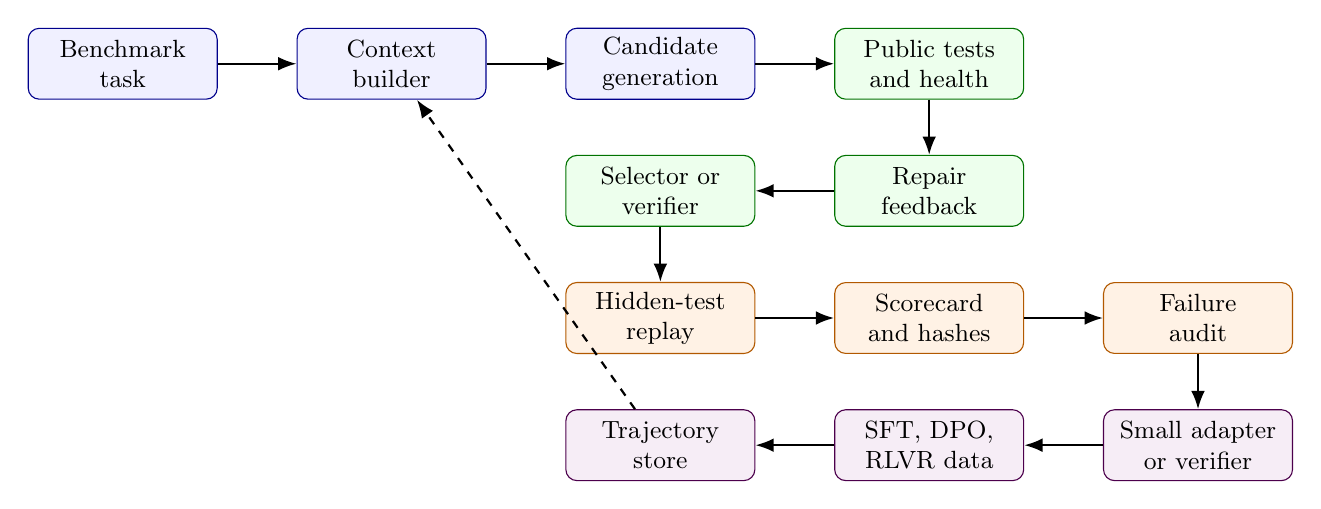
\begin{tikzpicture}[
    node distance=7mm and 10mm,
    box/.style={draw, rounded corners, align=center, minimum height=9mm, minimum width=24mm, font=\small},
    public/.style={box, fill=blue!6, draw=blue!55!black},
    verify/.style={box, fill=green!7, draw=green!45!black},
    audit/.style={box, fill=orange!10, draw=orange!70!black},
    train/.style={box, fill=violet!7, draw=violet!60!black},
    arrow/.style={-Latex, thick}
]
\node[public] (task) {Benchmark\\task};
\node[public, right=of task] (context) {Context\\builder};
\node[public, right=of context] (gen) {Candidate\\generation};
\node[verify, right=of gen] (publictest) {Public tests\\and health};
\node[verify, below=of publictest] (repair) {Repair\\feedback};
\node[verify, left=of repair] (selector) {Selector or\\verifier};
\node[audit, below=of selector] (hidden) {Hidden-test\\replay};
\node[audit, right=of hidden] (score) {Scorecard\\and hashes};
\node[audit, right=of score] (audit) {Failure\\audit};
\node[train, below=of hidden] (store) {Trajectory\\store};
\node[train, right=of store] (data) {SFT, DPO,\\RLVR data};
\node[train, right=of data] (adapter) {Small adapter\\or verifier};

\draw[arrow] (task) -- (context);
\draw[arrow] (context) -- (gen);
\draw[arrow] (gen) -- (publictest);
\draw[arrow] (publictest) -- (repair);
\draw[arrow] (repair) -- (selector);
\draw[arrow] (selector) -- (hidden);
\draw[arrow] (hidden) -- (score);
\draw[arrow] (score) -- (audit);
\draw[arrow] (audit) -- (adapter);
\draw[arrow] (adapter) -- (data);
\draw[arrow] (data) -- (store);
\draw[arrow, dashed] (store) -- (context);
\end{tikzpicture}
\caption{L20-CodeForge evaluation loop. Public signals drive generation,
selection, and repair. Private tests are reserved for final replay and audits.}
\label{fig:system}
\end{figure}

\section{Experiments}

\subsection{LiveCodeBench}

Table~\ref{tab:lcb-main} reports the main full-suite LiveCodeBench result. The
greedy baseline solves 297 of 1,055 tasks. Four-sample public-test selection
solves 378 tasks. Eight-sample selection solves 403 tasks, an absolute gain of
106 tasks over greedy decoding.

\begin{table}[H]
\centering
\begin{tabular}{llrrrr}
\toprule
Model & Protocol & Samples & Solved & Total & Pass@1 \\
\midrule
Qwen2.5-Coder-7B-Instruct & greedy & 1 & 297 & 1055 & 28.15 \\
Qwen2.5-Coder-7B-Instruct & public selection & 4 & 378 & 1055 & 35.83 \\
Qwen2.5-Coder-7B-Instruct & public selection & 8 & 403 & 1055 & 38.20 \\
\bottomrule
\end{tabular}
\caption{LiveCodeBench \texttt{release\_v6} full-suite results. Public
selection uses only visible public tests; hidden tests are used for final replay.}
\label{tab:lcb-main}
\end{table}

The gain is not uniform across difficulty levels. Easy tasks improve from 206
to 260 solved tasks, medium tasks from 82 to 124, and hard tasks from 9 to 19.
The hard-task result remains weak in absolute terms, which is consistent with
the need for stronger algorithmic candidates rather than only better selection.

\begin{table}[H]
\centering
\begin{tabular}{lrrrrr}
\toprule
Slice & Greedy solved & System solved & Total & Greedy & System \\
\midrule
Easy & 206 & 260 & 322 & 63.98 & 80.75 \\
Medium & 82 & 124 & 383 & 21.41 & 32.38 \\
Hard & 9 & 19 & 350 & 2.57 & 5.43 \\
\bottomrule
\end{tabular}
\caption{LiveCodeBench difficulty breakdown. Values in the last two columns are
percentages.}
\label{tab:lcb-breakdown}
\end{table}

\subsection{EvalPlus}

Table~\ref{tab:evalplus} reports the EvalPlus guardrail. The clean system rows
use public prompt and base-test signals, but not EvalPlus extra tests, for
selection. Both HumanEval+ and MBPP+ improve over greedy decoding.

\begin{table}[H]
\centering
\begin{tabular}{lrrrr}
\toprule
Dataset & Greedy base & System base & Greedy plus & System plus \\
\midrule
HumanEval & 89.0 & 98.2 & 84.8 & 92.7 \\
MBPP & 82.8 & 96.0 & 72.2 & 81.7 \\
\bottomrule
\end{tabular}
\caption{EvalPlus results. Values are pass@1 percentages. The plus columns use
the stricter EvalPlus tests for scoring, not for candidate selection.}
\label{tab:evalplus}
\end{table}

\subsection{X-Coder Control Slice}

We also probed IIGroup/X-Coder-RL-Qwen2.5-7B on a medium-difficulty control
slice. Automatic and strict starter-prefix checks both scored 0/12. Public-only
second-pass repair reached 2/12. A single public-feedback repair round reached
4/12. A second public-feedback round produced visible-test signal but no hidden
passes. We therefore treat the first feedback round as useful but not sufficient
for broad claims.

\section{Failure Analysis}

The main failure class on the eight-sample LiveCodeBench run is wrong answer,
not syntax or missing entrypoints. This suggests that future work should
prioritize better algorithmic candidates and stronger verifier calibration over
format-only prompting.

Several attempted improvements did not hold up under hidden replay. Repeated
public-feedback repair overfit visible tests on the second round. Input-only
differential fuzzing improved candidate-pair coverage on some targets but did
not change selection when the pool contained too few public-passing alternatives. An
expected-output verifier over generated inputs regressed the targeted replay,
indicating that verifier confidence needs calibration before it can safely alter
headline selections.

\section{Reproducibility}

The repository includes committed benchmark summaries, saved generations,
reports, hash manifests, and CI checks. The full hidden-test LiveCodeBench JSONL
is not committed. Instead, the repository records materialization commands,
source hashes, generation hashes, evaluator outputs, and compact summaries.

For the main LiveCodeBench result, the committed summary hash is:

\begin{center}
\small
\texttt{2a0ff919aa15eb9ecdf74824f7bf790a23f6d0197ef74970b6190c60e0e00772}
\end{center}

The generalization scorecard hash is:

\begin{center}
\small
\texttt{1eb0402378ea25732225b29d7ba367b6111ab3351e54cc7c01fa7646a7a12712}
\end{center}

The repository also includes a separate reproducibility document with expected
command outputs and artifact-hash checks.

\section{Limitations}

The strongest limitation is that the main gain is a system-level gain, not a
model-weight gain. The eight-sample selector is useful in practice but should
not be confused with a greedy checkpoint improvement. The experiments also use
one main base model and one main GPU type. Public tests are legitimate solver
signals, but repeated repair on public failures can overfit them. Finally,
private benchmark tests cannot be committed directly, so full hidden replay
requires local materialization of the benchmark payload.

\section{Conclusion}

L20-CodeForge shows that a careful single-GPU system can extract a meaningful
amount of additional coding performance from a 7B open model while preserving a
clean benchmark boundary. The useful parts are not only the positive results,
but also the audit trail: public selection helps, first-round repair can help,
and several plausible verifier variants fail without calibration. The next step
is to convert this infrastructure into a verified-data and RLVR pipeline that
improves single-sample model behavior on held-out tasks.

\bibliographystyle{plainnat}
\bibliography{references}

\end{document}
